%%%%%%%%%%%%%%%%%%%%%%%%%%%%%%%%%%%%%%%%%
% kaobook
% LaTeX Template
% Version 1.2 (4/1/2020)
%
% This template originates from:
% https://www.LaTeXTemplates.com
%
% For the latest template development version and to make contributions:
% https://github.com/fmarotta/kaobook
%
% Authors:
% Federico Marotta (federicomarotta@mail.com)
% Based on the doctoral thesis of Ken Arroyo Ohori (https://3d.bk.tudelft.nl/ken/en)
% and on the Tufte-LaTeX class.
% Modified for LaTeX Templates by Vel (vel@latextemplates.com)
%
% License:
% CC0 1.0 Universal (see included MANIFEST.md file)
%
%%%%%%%%%%%%%%%%%%%%%%%%%%%%%%%%%%%%%%%%%

%----------------------------------------------------------------------------------------
%	PACKAGES AND OTHER DOCUMENT CONFIGURATIONS
%----------------------------------------------------------------------------------------

\documentclass[
	fontsize=10pt, % Base font size
	twoside=false, % Use different layouts for even and odd pages (in particular, if twoside=true, the margin column will be always on the outside)
	%open=any, % If twoside=true, uncomment this to force new chapters to start on any page, not only on right (odd) pages
	%chapterprefix=true, % Uncomment to use the word "Chapter" before chapter numbers everywhere they appear
	chapterentrydots=true, % Uncomment to output dots from the chapter name to the page number in the table of contents
	numbers=noenddot, % Comment to output dots after chapter numbers; the most common values for this option are: enddot, noenddot and auto (see the KOMAScript documentation for an in-depth explanation)
	%draft=true, % If uncommented, rulers will be added in the header and footer
	%overfullrule=true, % If uncommented, overly long lines will be marked by a black box; useful for correcting spacing problems
]{kaobook}
\renewcommand\thesection{\arabic{section}}
\renewcommand\thesubsection{\arabic{section}.\arabic{subsection}}
%!TEX root = ../thesis.tex

%\hypersetup{colorlinks,linktocpage,urlcolor=red}
%
%\definecolor{myGreen}{HTML}{05C18E} 
%\definecolor{myGreenDarker}{HTML}{178C6C} \colorlet{mylinkcolor}{green!50!black}

\definecolor{webbrown}{rgb}{.6,0,0}

\hypersetup{
  colorlinks=true,
  linkcolor=black, %myGreenDarker
%  urlcolor=myGreenDarker,
  citecolor = webbrown,
  urlcolor=webbrown,
  hyperfootnotes=false,
  hypertexnames,
  bookmarks=true}
  
%\setsidenotefont{\color{black}\footnotesize}   <-- set the color and font here
%\setmarginnotefont{\color{black}\footnotesize} <-- and here
%
%\renewcommand{\maketitlepage}[0]{%
%  \cleardoublepage%
%  {%
%  \sffamily%
%  \begin{fullwidth}%
%  \fontsize{18}{20}\selectfont\par\noindent\textcolor{darkgray}{\allcaps{\thanklessauthor}}%
%  \vspace{11.5pc}%
%  \fontsize{24}{45}\selectfont\par\noindent\textcolor{darkgray}{\allcaps{\thanklesstitle}}
%  \fontsize{17.4}{25}\selectfont\par\noindent\textcolor{darkgray}{\allcaps{For Affective Touch Communication}}%
%  \fontsize{10.0}{17}\selectfont\par\noindent\textcolor{Gray}{\allcaps{Devices that touch to convey emotions and feel that contact}}%
%
%  \vfill%
%  \fontsize{14}{16}\selectfont\par\noindent\allcaps{\thanklesspublisher}%
%  \end{fullwidth}%
%  }
 %  \thispagestyle{empty}%
%  \clearpage%
%}

%%%% Kevin Godny's code for title page and contents from https://groups.google.com/forum/#!topic/tufte-latex/ujdzrktC1BQ
% \makeatletter
% \renewcommand{\maketitlepage}{%
% \begingroup%
% \setlength{\parindent}{0pt}

% {\fontsize{24}{24}\selectfont\textit{\@author}\par}

% \vspace{1.75in}{\fontsize{36}{54}\selectfont\@title\par}

% % \vspace{0.5in}{\fontsize{14}{14}\selectfont\textsf{\smallcaps{\@date}}\par}
% \vspace{0.5in}{\fontsize{14}{14}\selectfont\textsf{\sc\@date}\par}

% \vfill{\fontsize{14}{14}\selectfont\textit{\@publisher}\par}

% \thispagestyle{empty}
% \endgroup
% }
% \makeatother

%\titlecontents{part}%
%    [0pt]% distance from left margin
%    {\addvspace{0.25\baselineskip}}% above (global formatting of entry)
%    {\allcaps{Part~\thecontentslabel}\allcaps}% before w/ label (label = ``Part I'')
%    {\allcaps{Part~\thecontentslabel}\allcaps}% before w/o label
%    {}% filler and page (leaders and page num)
%    [\vspace*{0.5\baselineskip}]% after
%
%
%\titlecontents{chapter}%
%    [4em]% distance from left margin
%    {}% above (global formatting of entry)
%    {\contentslabel{2em}\textit}% before w/ label (label = ``Chapter 1'')
%    {\hspace{0em}\textit}% before w/o label
%    {\qquad\thecontentspage}% filler and page (leaders and page num)
%    [\vspace*{0.5\baselineskip}]% after
%%%%% End additional code by Kevin Godby


%% CHANGE CITE COMMAND
\renewcommand{\cite}[1]{%
~\citep{#1}%
}



%%
% If they're installed, use Bergamo and Chantilly from www.fontsite.com.
% They're clones of Bembo and Gill Sans, respectively.
%\IfFileExists{bergamo.sty}{\usepackage[osf]{bergamo}}{}% Bembo
%\IfFileExists{chantill.sty}{\usepackage{chantill}}{}% Gill Sans

%%%%%%%%%%%%%%%%%%%%%%%%%%%%%%%%%%%%%%%%%%%%%%%%%%%%%%%%%%
%%% INCLUSION / EXCLUSION %%%%%%%%%%%%%%%%%%%
\usepackage{microtype}
\usepackage{comment}
% !!! Comment or uncomment line under to exclude or include the content of the chapter:
%\excludecomment{content} % exclude the content, (only get introduction and summary)
\includecomment{content} % include the content, (get eveevolutionrything)
\includecomment{export}
%%%%%%%%%%%%%%%%%%%%%%%%%%%%%%%%%%%%%%%%%%%%%%%%%%%%%%%%%%


%%
% For nicely typeset tabular material
\usepackage{booktabs}
%%
% For graphics / images
\usepackage{graphicx}
\setkeys{Gin}{width=\linewidth,totalheight=\textheight,keepaspectratio}
\graphicspath{{graphics/}}
% The fancyvrb package lets us customize the formatting of verbatim environments.  We use a slightly smaller font.
\usepackage{fancyvrb}
\fvset{fontsize=\normalsize}

%%
% Prints argument within hanging parentheses (i.e., parentheses that take
% up no horizontal space).  Useful in tabular environments.
% \newcommand{\hangp}[1]{\makebox[0pt][r]{(}#1\makebox[0pt][l]{)}}

%%
% Prints an asterisk that takes up no horizontal space.
% Useful in tabular environments.
% \newcommand{\hangstar}{\makebox[0pt][l]{*}}

%%
% Prints a trailing space in a smart way.
\usepackage{xspace}

%
%%%
%% Some shortcuts for Tufte's book titles.  The lowercase commands will
%% produce the initials of the book title in italics.  The all-caps commands
%% will print out the full title of the book in italics.
%\newcommand{\vdqi}{\textit{VDQI}\xspace}
%\newcommand{\ei}{\textit{EI}\xspace}
%\newcommand{\ve}{\textit{VE}\xspace}
%\newcommand{\be}{\textit{BE}\xspace}
%%\newcommand{\VDQI}{\textit{Visualizing dynamic social data  with rationally designed constructive systems}\xspace}
%\newcommand{\EI}{\textit{Envisioning Information}\xspace}
%\newcommand{\VE}{\textit{Visual Explanations}\xspace}
%\newcommand{\BE}{\textit{Beautiful Evidence}\xspace}
%\newcommand{\TL}{Tufte-\LaTeX\xspace}

% Prints the month name (e.g., January) and the year (e.g., 2008)
% \newcommand{\monthyear}{%
%   \ifcase\month\or January\or February\or March\or April\or May\or June\or
%   July\or August\or September\or October\or November\or
%   December\fi\space\number\year
% }





% Prints an epigraph and speaker in sans serif, all-caps type.
\newcommand{\openepigraph}[2]{%
  %\sffamily\fontsize{14}{16}\selectfont
  \begin{fullwidth}
  \sffamily\large
  \begin{doublespace}
  \noindent\allcaps{#1}\\% epigraph
  \noindent\allcaps{#2}% author
  \end{doublespace}
  \end{fullwidth}
}

% Inserts a blank page
% \newcommand{\blankpage}{\newpage\hbox{}\thispagestyle{empty}\newpage}

\usepackage{units}

% Typesets the font size, leading, and measure in the form of 10/12x26 pc.
\newcommand{\measure}[3]{#1/#2$\times$\unit[#3]{pc}}

% Macros for typesetting the documentation
\newcommand{\hlred}[1]{\textcolor{Green}{#1}}% prints in red
\newcommand{\hangleft}[1]{\makebox[0pt][r]{#1}}
% \newcommand{\hairsp}{\hspace{1pt}}% hair space
\newcommand{\hquad}{\hskip0.5em\relax}% half quad space
\newcommand{\TODO}{\textcolor{red}{\bf TODO!}\xspace}
% \newcommand{\ie}{\textit{i.\hairsp{}e.}\xspace}
% \newcommand{\eg}{\textit{e.\hairsp{}g.}\xspace}
% \newcommand{\na}{\quad--}% used in tables for N/A cells
\providecommand{\XeLaTeX}{X\lower.5ex\hbox{\kern-0.15em\reflectbox{E}}\kern-0.1em\LaTeX}
\newcommand{\tXeLaTeX}{\XeLaTeX\index{XeLaTeX@\protect\XeLaTeX}}
% \index{\texttt{\textbackslash xyz}@\hangleft{\texttt{\textbackslash}}\texttt{xyz}}
\newcommand{\tuftebs}{\symbol{'134}}% a backslash in tt type in OT1/T1
\newcommand{\doccmdnoindex}[2][]{\texttt{\tuftebs#2}}% command name -- adds backslash automatically (and doesn't add cmd to the index)
\newcommand{\doccmddef}[2][]{%
  \hlred{\texttt{\tuftebs#2}}\label{cmd:#2}%
  \ifthenelse{\isempty{#1}}%
    {% add the command to the index
      \index{#2 command@\protect\hangleft{\texttt{\tuftebs}}\texttt{#2}}% command name
    }%
    {% add the command and package to the index
      \index{#2 command@\protect\hangleft{\texttt{\tuftebs}}\texttt{#2} (\texttt{#1} package)}% command name
      \index{#1 package@\texttt{#1} package}\index{packages!#1@\texttt{#1}}% package name
    }%
}% command name -- adds backslash automatically
\newcommand{\doccmd}[2][]{%
  \texttt{\tuftebs#2}%
  \ifthenelse{\isempty{#1}}%
    {% add the command to the index
      \index{#2 command@\protect\hangleft{\texttt{\tuftebs}}\texttt{#2}}% command name
    }%
    {% add the command and package to the index
      \index{#2 command@\protect\hangleft{\texttt{\tuftebs}}\texttt{#2} (\texttt{#1} package)}% command name
      \index{#1 package@\texttt{#1} package}\index{packages!#1@\texttt{#1}}% package name
    }%
}% command name -- adds backslash automatically
\newcommand{\docopt}[1]{\ensuremath{\langle}\textrm{\textit{#1}}\ensuremath{\rangle}}% optional command argument
\newcommand{\docarg}[1]{\textrm{\textit{#1}}}% (required) command argument
\newenvironment{docspec}{\begin{quotation}\ttfamily\parskip0pt\parindent0pt\ignorespaces}{\end{quotation}}% command specification environment
\newcommand{\docenv}[1]{\texttt{#1}\index{#1 environment@\texttt{#1} environment}\index{environments!#1@\texttt{#1}}}% environment name
\newcommand{\docenvdef}[1]{\hlred{\texttt{#1}}\label{env:#1}\index{#1 environment@\texttt{#1} environment}\index{environments!#1@\texttt{#1}}}% environment name
\newcommand{\docpkg}[1]{\texttt{#1}\index{#1 package@\texttt{#1} package}\index{packages!#1@\texttt{#1}}}% package name
\newcommand{\doccls}[1]{\texttt{#1}}% document class name
\newcommand{\docclsopt}[1]{\texttt{#1}\index{#1 class option@\texttt{#1} class option}\index{class options!#1@\texttt{#1}}}% document class option name
\newcommand{\docclsoptdef}[1]{\hlred{\texttt{#1}}\label{clsopt:#1}\index{#1 class option@\texttt{#1} class option}\index{class options!#1@\texttt{#1}}}% document class option name defined
\newcommand{\docmsg}[2]{\bigskip\begin{fullwidth}\noindent\ttfamily#1\end{fullwidth}\medskip\par\noindent#2}
\newcommand{\docfilehook}[2]{\texttt{#1}\index{file hooks!#2}\index{#1@\texttt{#1}}}
\newcommand{\doccounter}[1]{\texttt{#1}\index{#1 counter@\texttt{#1} counter}}




%\geometry{textwidth=.55\paperwidth}


% Generates the index
\usepackage{makeidx}
\makeindex



% Nomenclature
%\usepackage{nomencl}
%\renewcommand{\nomname}{List of Abbreviations}
%\makenomenclature



%%%%
\makeatletter
\renewcommand*\l@figure{\@dottedtocline{1}{1.5em}{2.3em}}
\makeatother

%% change TOC
\setcounter{tocdepth}{2}
\setcounter{secnumdepth}{2}

%%%%%%%%%%%%%%%%%%%%%%%%%%%%%%%%%%%%%%%%%%%%%%%%%%
%%%%%%%%%%%%%%%%%%%%%%%%%%%%%%%%%%%%%%%%%%%%%%%%%%
\let\Bbbk\relax
\usepackage{amssymb}% http://ctan.org/pkg/amssymb
\usepackage{pifont}% http://ctan.org/pkg/pifont
%\usepackage{graphics} % for EPS, load graphicx instead
\usepackage{graphicx}
\usepackage{multirow}
\usepackage{xspace}
\usepackage{tabularx}
\usepackage{color}
\usepackage{listings}
\usepackage{ulem}
\usepackage{colortbl}
\usepackage{morefloats}
\usepackage{enumitem}
\usepackage{rotating}
\usepackage{comment}
\usepackage{rotating}
% \usepackage[sort, numbers]{natbib} 
\usepackage[retainorgcmds]{IEEEtrantools}
\usepackage{bibentry}
\usepackage{longtable}
\usepackage{glossaries}
\usepackage{gensymb}
\usepackage{csvsimple}
\usepackage{amsmath}
\usepackage{cleveref}% Has to be loaded after hyperref
\usepackage[utf8]{inputenc}
\usepackage{todonotes}
\usepackage{marginfix}
\usepackage[export]{adjustbox}
\usepackage{fullwidth}
%\setkeys{Gin}{height=2cm}
%\usepackage{float}
\usepackage[caption=false]{subfig}

\usepackage[strict]{changepage}

\setlist[description]{style = multiline, labelwidth = 55pt}
\usepackage[parfill]{parskip}
\makeatletter
% Paragraph indentation and separation for normal text
% \renewcommand{\@tufte@reset@par}{%
%   \setlength{\RaggedRightParindent}{1.0pc}%
%   \setlength{\parindent}{1pc}%
%   \setlength{\parskip}{8pt}%\baselineskip % default 12pt for 10pt font
% }
% \@tufte@reset@par

% Paragraph indentation and separation for marginal text
% \renewcommand{\@tufte@margin@par}{%
%   \setlength{\RaggedRightParindent}{0.5pc}%
%   \setlength{\JustifyingParindent}{0.0pc}%
%   \setlength{\parindent}{0.5pc}%
%   \setlength{\parskip}{6pt}%
% }
\makeatother





%% Correction

%\newcommand{\Ssubsection}[1]{{\setlength{\parindent}{0cm}\normalfont{\textit{\newline#1}}}\newline}
%\newcommand{\Ssubsection}[1]{{\setlength{\parindent}{0cm}\normalfont{\textit{#1}}}}




\usepackage{mdframed}
\newmdenv[
  leftmargin = 0pt,
  innerleftmargin = 1em,
  innerrightmargin = 0pt,
 innerbottommargin = 0pt,
  innertopmargin = 0pt,
  rightmargin = 0pt,
  linewidth = 2pt,
  topline = false,
  rightline = false,
  bottomline = false,
  skipabove = 6pt
  ]{leftbar}


\newcommand{\mframe}[1]{\begin{leftbar}{#1}\end{leftbar}}


%You can copy those commands to the preamble of your document and fill in the values that you prefer (e.g., 0pt for the indents and \baselineskip for the \parskip).








% \titleclass{\subsubsection}{straight}
% \titleformat{\subsubsection}%
%   [hang]% shape
%   {\normalfont\large\itshape}% format applied to label+text
%   {\thesubsubsection}% label
%   {1em}% horizontal separation between label and title body
%   {}% before the title body
%   []% after the title body
  
  
  

%%%%%%%%%%%%%%%%%%%%%%%%%%%%%%%%%%%%%
%%%%%% FANCY FRAMES
%% https://tex.stackexchange.com/questions/348501/example-of-box-inside-box
%%%%%%%%%%%%%%%%%%%%%%%%
%\usepackage[margin=0.5in]{geometry}
%\usepackage{tikz,lipsum,lmodern}
\usepackage{tikz,lipsum}
\usepackage[most]{tcolorbox}

\tcbset{titre/.style={boxed title style={boxrule=0pt,colframe=white}}}

\definecolor{gradientGreenL}{HTML}{1fe2ad} 
\definecolor{gradientGreenR}{HTML}{d4eb6f} 


\newtcolorbox{BoxResume}[2][]{
                boxrule=0.5pt,
                colback=white,
                top=3pt,bottom=2pt,left=2pt,right=2pt,
                colframe=webbrown,
                fonttitle=\sffamily\small,%\bfseries
                coltitle=black,
                colbacktitle=white,
                enhanced,
                attach boxed title to top left={xshift=5mm, yshift=-2mm},
                title=#2,#1
                }


\newtcolorbox{BoxIn}{
enhanced,
colframe=white,
interior style={
left color=gradientGreenL!7!white,
right color=gradientGreenR!7!white},
%frame style image=background\aa.jpg
left=5mm,
top=4mm,
bottom=4mm,
right=5mm,
boxsep=0mm,
nobeforeafter}



\newtcolorbox{BoxResumeNew}[2][]{
                boxrule=1pt,
                colback=white,
                top=3pt,bottom=2pt,left=2pt,right=2pt,
                colframe=black,
                fonttitle=\sffamily\small,%\bfseries
                coltitle=black,
                colbacktitle=white,
                enhanced,
                attach boxed title to top left={xshift=5mm, yshift=-2mm},
                title=#2,#1
                }


\newtcolorbox{BoxInNew}{
enhanced,
colframe=white,
colback=black!2!white,
%frame style image=background\aa.jpg
left=5mm,
top=4mm,
bottom=4mm,
right=5mm,
boxsep=0mm,
nobeforeafter}



\newcommand{\remember}[1]{
\vspace*{\fill}
\begin{BoxResumeNew}[titre]{WHAT YOU MUST REMEMBER}
 \begin{BoxInNew}{}
 #1
 \end{BoxInNew}{}
\end{BoxResumeNew}
\vspace{0.5cm}
} 

%%%% USAGE

%\remember{
%\textit{Contributions:}\vspace{0.5em}
%\begin{itemize}
%\item[$-$] Design and development of a finger robotic actuator for mobile devices
%\item[$-$] Applications and scenarios that demonstrate its use as a medium,  as a tool and as a virtual partner
%\item[$-$] Initial evaluation of perception of the appearance and the relevance of scenarios
%\end{itemize}
%}


%%%%%%%%%%%%%%%%%%%%%%%%%%%%%%
%%%%%%%%%   QUOTE %%%%%%%%%%%%%%%%%%%
%%%%%%%%%%%%%%%%%%

\makeatletter
\renewcommand{\@chapapp}{}% Not necessary...
\newenvironment{chapquote}[2][2em]
  {\setlength{\@tempdima}{#1}%
   \def\chapquote@author{#2}%
   \parshape 1 \@tempdima \dimexpr\textwidth-2\@tempdima\relax%
   }
  {\par\normalfont\hfill--\ \chapquote@author\hspace*{\@tempdima}\par\bigskip}
\makeatother


%\listfiles

% Set the language
\usepackage[english]{babel} % Load characters and hyphenation
\usepackage[english=british]{csquotes} % English quotes

% Load packages for testing
% \usepackage{blindtext}
%\usepackage{showframe} % Uncomment to show boxes around the text area, margin, header and footer
%\usepackage{showlabels} % Uncomment to output the content of \label commands to the document where they are used

% Load the bibliography package
\usepackage{styles/kaobiblio}
\addbibresource{main.bib} % Bibliography file

% Load mathematical packages for theorems and related environments. NOTE: choose only one between 'mdftheorems' and 'plaintheorems'.
% \usepackage{styles/mdftheorems}
\usepackage{styles/plaintheorems}

\graphicspath{{examples/documentation/images/}{images/}} % Paths in which to look for images

\makeindex[columns=3, title=Alphabetical Index, intoc] % Make LaTeX produce the files required to compile the index

\makeglossaries% Make LaTeX produce the files required to compile the glossary

\makenomenclature% Make LaTeX produce the files required to compile the nomenclature

% Reset sidenote counter at chapters
%\counterwithin*{sidenote}{chapter}

%----------------------------------------------------------------------------------------

\newcommand{\red}[1]{\textcolor[rgb]{1, 0, 0}{#1}}


\begin{document}

%----------------------------------------------------------------------------------------
%	BOOK INFORMATION
%----------------------------------------------------------------------------------------

% \titlehead{The \texttt{kaobook} class}
\subject{Master Thesis}
\title{Swarm Drones Control Platform}
\subtitle{A modular and scalable platform for swarm drone control}


\author{Nicolas Leboucher}

\date{\today}

\titlehead{\centering
\includegraphics[width=6cm]{dvic.png}}

\publishers{\textbf{Supervisors}\\ Dr Xiao Xiao and Dr Marc Teyssier Professor at IFT }


%----------------------------------------------------------------------------------------

\frontmatter % Denotes the start of the pre-document content, uses roman numerals

%----------------------------------------------------------------------------------------
%	OPENING PAGE
%----------------------------------------------------------------------------------------

% \makeatletter
% \extratitle{
% 	% In the title page, the title is vspaced by 9.5\baselineskip
% 	\vspace*{9\baselineskip}
% 	\vspace*{\parskip}
% 	\begin{center}
% 		% In the title page, \huge is set after the komafont for title
% 		\usekomafont{title}\huge\@title
% 	\end{center}
% }
% \makeatother

%----------------------------------------------------------------------------------------
%	COPYRIGHT PAGE
%----------------------------------------------------------------------------------------

% \makeatletter
% \uppertitleback{\@titlehead} % Header

% \lowertitleback{
% 	\textbf{Disclaimer}\\
% 	You can edit this page to suit your needs. For instance, here we have a no copyright statement, a colophon and some other information. This page is based on the corresponding page of Ken Arroyo Ohori's thesis, with minimal changes.
	
% 	\medskip
	
% 	\textbf{No copyright}\\
% 	\cczero\ This book is released into the public domain using the CC0 code. To the extent possible under law, I waive all copyright and related or neighbouring rights to this work.
	
% 	To view a copy of the CC0 code, visit: \\\url{http://creativecommons.org/publicdomain/zero/1.0/}
	
% 	\medskip
	
% 	\textbf{Colophon} \\
% 	This document was typeset with the help of \href{https://sourceforge.net/projects/koma-script/}{\KOMAScript} and \href{https://www.latex-project.org/}{\LaTeX} using the \href{https://github.com/fmarotta/kaobook/}{kaobook} class.
	
% 	The source code of this book is available at:\\\url{https://github.com/fmarotta/kaobook}
	
% 	(You are welcome to contribute!)
	
% 	\medskip
	
% 	\textbf{Publisher} \\
% 	First printed in May 2019 by \@publishers
% }
% \makeatother

%----------------------------------------------------------------------------------------
%	DEDICATION
%----------------------------------------------------------------------------------------

% \dedication{
% 	The harmony of the world is made manifest in Form and Number, and the heart and soul and all the poetry of Natural Philosophy are embodied in the concept of mathematical beauty.\\
% 	\flushright -- D'Arcy Wentworth Thompson
% }

%----------------------------------------------------------------------------------------
%	OUTPUT TITLE PAGE AND PREVIOUS
%----------------------------------------------------------------------------------------

% Note that \maketitle outputs the pages before here

% If twoside=false, \uppertitleback and \lowertitleback are not printed
% To overcome this issue, we set twoside=semi just before printing the title pages, and set it back to false just after the title pages
\KOMAoptions{twoside=semi}
\maketitle
\KOMAoptions{twoside=false}



%----------------------------------------------------------------------------------------
%	TABLE OF CONTENTS & LIST OF FIGURES/TABLES
%----------------------------------------------------------------------------------------

\begingroup % Local scope for the following commands

% Define the style for the TOC, LOF, and LOT
%\setstretch{1} % Uncomment to modify line spacing in the ToC
% \hypersetup{linkcolor=blue} % Uncomment to set the colour of links in the ToC
\setlength{\textheight}{23cm} % Manually adjust the height of the ToC pages

% Turn on compatibility mode for the etoc package
\etocstandarddisplaystyle % "toc display" as if etoc was not loaded
\etocstandardlines % toc lines as if etoc was not loaded

% Comment both of the following lines to have the LOF and the LOT on different pages
\let\cleardoublepage\bigskip
\let\clearpage\bigskip

% \listoftables % Output the list of tables





\endgroup

%----------------------------------------------------------------------------------------
%	MAIN BODY
%----------------------------------------------------------------------------------------

\mainmatter % Denotes the start of the main document content, resets page numbering and uses arabic numbers
\setchapterstyle{kao} % Choose the default chapter heading style
\clearpage
\phantomsection
\tableofcontents
% add introduction to the table of contents and conclusion
\section{Introduction}

\subsection{Background and Motivation}

Swarm robotics is an emerging field in robotics inspired by biological systems, such as flocks of birds or colonies of ants, where simple units collaborate to achieve complex tasks. In recent years, advancements in drone technology have expanded the potential applications of swarm robotics, including environmental monitoring, search-and-rescue operations, and industrial automation \cite{swarm_survey}. In particular, drones operating as swarms offer a promising solution for tasks requiring adaptability and scalability.

One key area of interest is the integration of drone swarms into environments shared with humans. Applications such as drone-based assistance systems in healthcare, smart warehouses, and collaborative robotics emphasize the need for reliable, safe human-drone interaction \cite{swarm_survey}. The use of drones in indoor environments, where traditional positioning systems such as GPS are not viable, presents both opportunities and challenges, particularly when human safety and interaction are prioritized.

In this context, existing swarm control platforms like Crazyswarm and CFlib offer robust tools for drone coordination and control. However, these platforms often require specialized equipment, such as motion capture systems, and rely on Python-based libraries, limiting accessibility for non-expert users and those working in non-research settings \cite{crazyflie,bitcraze_cflib}. This raises a gap: a need for more accessible, intuitive control systems that allow seamless interaction between human operators and drone swarms in real-time indoor environments.

\subsection{Problem Statement}

While existing platforms provide powerful tools for swarm control, they do not address the challenge of creating a system that integrates human pose detection with real-time drone control in a user-friendly and accessible way. Most current systems are limited in their ability to allow developers to work directly with drones in environments where they need to safely interact with human operators.

This research addresses this gap by proposing a web-based platform for controlling swarms of Crazyflie drones in indoor spaces using real-time human pose estimation. The platform aims to enable intuitive and responsive interaction between humans and drones without requiring complex external systems.

We want to have our scene of drones including our operators and drones. Similarly in red is the drone system and in yellow the human system with the human pose detection. In red above there is the drone localization system. In grey above is the human localization system.

\begin{figure}[htbp]
    \centerline{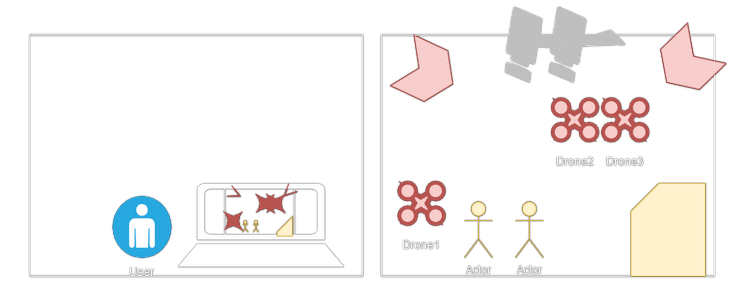
\includegraphics{images/setting.png}}
    \caption{ Our setup for controlling drones indoors around humans. Similarly in red is the drone system and in yellow the human system with the human pose detection. In red above there is the drone localization system. In grey above is the human localization system. }
    \label{fig}
    \end{figure}

\subsection{Research Objectives}

This research aims to address the limitations of existing swarm control platforms by developing a user-friendly, web-based system for controlling swarms of drones in indoor environments where interaction with humans is required. The main objectives of this research are as follows:

\begin{itemize}
    \item Develop a web-based platform for controlling swarms of Crazyflie drones, enabling easier access for developers, researchers, and non-experts.
    \item Integrate real-time human pose detection using affordable and accessible technologies, such as Intel RealSense and MediaPipe \cite{realsense_mediapipe}.
    \item Ensure safe and responsive drone interactions in indoor environments by integrating collision avoidance systems and real-time feedback.
    \item Evaluate the platform's performance in both controlled and dynamic indoor environments with human interaction.
\end{itemize}

This research will demonstrate how a web-based interface, coupled with advanced human pose detection, can make drone swarm control more accessible and enhance human-drone collaboration in shared spaces.

\subsection{Significance of the Research}

The proposed platform has the potential to significantly impact the field of swarm robotics by broadening access to swarm control technologies. Currently, systems like \textit{CrazySwarm} and \textit{CFLib} require Python-based development, which limits their use to researchers or developers with specific technical expertise \cite{crazyflie,bitcraze_cflib}. By shifting to a web-based architecture, this research will make drone control systems more accessible to a wider audience, enabling cross-platform development and more intuitive interfaces.

Furthermore, by integrating real-time human pose detection, this platform introduces a novel method for enabling drones to interact with humans safely in indoor environments. This has wide-ranging applications, from smart warehouses, where drones assist human workers \cite{flyjacket, human_drone_interaction}. The platform also has the potential to be used in educational settings, allowing students to interact with drones without complex technical setups.

Ultimately, this research fills a critical gap in current swarm robotics systems, creating a foundation for future development in both research and practical applications, particularly in areas where drone-human interaction is necessary.

\subsection{Scope and Limitations}

The proposed platform has limitations that should be considered. First, the platform is designed for indoor environments, where GPS signals are unreliable, and human interaction is a primary concern. It can not work outdoors.

The platform will not adress internal positioning of the drones, only external positioning.

The platform will not address drone swarm control in outdoor or GPS-based environments.

The platform will use real-time human pose detection technologies like Intel RealSense and MediaPipe, which may have limitations in complex environments.

Despite these limitations, the proposed platform offers a significant advancement in swarm robotics by providing a user-friendly interface for controlling drones in indoor environments around humans. The platform's focus on accessibility and safety makes it a valuable tool for researchers, developers, and educators interested in swarm robotics and human-drone interaction.

\subsection{Structure Overview}
    Chapter 1 will review the State of the Art, including existing swarm control platforms like CrazySwarm, ModQuad, and human pose detection systems.

    Chapter 2 will describe the design and implementation of the proposed Drone Control Kernel.

    Chapter 3 Will describe the integration of real-time human pose detection.

    Chapter 4 will present the platform for human-swarm interaction will present the experimental setup and results, validating the platform's functionality including possible extensions of the platform for larger-scale deployment.

    Chapter 5 will discuss the conclusions

% \subsection*{Motivation}
% \subsubsection*{Overview of Swarm Robotics}


% We present a novel platform for controlling swarms of Crazyfly drones that utilizes more user-friendly technology compared to the existing Python CFlib controller. This approach demonstrates the feasibility and potential of safely operating drones around humans in indoor environments. By leveraging accessible interfaces, our platform aims to make more accessible Human-Drone technologies using widely used web technologies.
% Swarm robotics has garnered significant attention in recent years due to its applications in environmental monitoring, agriculture, and search-and-rescue missions. Among swarm robotics, drone swarms present unique challenges and opportunities, particularly in dynamic environments such as indoor spaces where interaction with humans becomes crucial. The ability to control multiple drones simultaneously and safely around humans is essential for realizing the full potential of swarm robotics in various applications. 
% However, existing platforms for controlling drone swarms often lack the necessary integration with human interaction.

% While several platforms exist for drone swarm control, such as CrazySwarm and CFLib, none provides an accessible, web-based system for controlling swarms in indoor environments with human interaction. This gap limits the deployment of drone swarms in shared spaces such as hospitals, warehouses, or educational environments. Our platform addresses this gap by providing a user-friendly interface for controlling drone swarms around humans indoors. By leveraging web technologies, we aim to democratize drone swarm control and enable developers to create innovative applications that combine human interaction. As we are in a research environment we are able to test and develop this platform in a safe environment. We are able to test the platform with known people and subjects. We plan on testing it further and giving it to students to test further and develop on. This technology gives possibilities in development to warehouses for adding drone carriers around sensitive objects or animals.

% Our technological platform is based on the Crazyflie UAVs, which are widely used in research and educational settings due to their small size, agility, and open-source software. By developing a web-based interface for controlling these drones, we aim to lower the barrier to entry for developers and researchers interested in swarm robotics. Our platform integrates real-time human pose detection and collision avoidance to ensure safe operation of drone swarms around humans. This integration enables developers to create interactive applications that leverage human-drone interaction in indoor environments.

% For this we have 5 crazyflie drones that 


\begin{marginfigure}[-5cm] % Adjust the vertical placement
    \centering
    \includegraphics[width=\linewidth]{images/plastic-waste.png}
    \caption{Plastics pollution on a beach}
    \label{fig:plastics}
\end{marginfigure}
% annoncer le plan et resumer les parties en quelques lignes
\section{State of the Art}
% ajouter 
In recent years, swarm drone technology has advanced significantly, leading to breakthroughs in human-drone interaction and multi-robot systems. While several research efforts have focused on the safety, control, and interaction between drones and humans, there remains a gap in the availability of robust platforms for developers to control drone swarms indoors around humans. This section will explore existing works that demonstrate safe operation of drones around humans, systems that enable real-time drone control based on human input, and the identified gaps in the current technological landscape.

\subsection{Safe Drone Flight Around Humans}

Safety is a primary concern when operating drones in close proximity to humans, especially in confined spaces such as indoor environments. Several research efforts have focused on ensuring that drones can operate around humans without posing significant risks.

One such project is Drone \& Me, which investigates how drones can safely navigate around humans by recognizing human poses and responding accordingly \cite{drone_me}. In addition, Ju et al. (2017) proposed real-time trajectory adjustments for drones to ensure safe flight paths when operating around humans indoors. These systems emphasize the importance of autonomous collision avoidance and the use of protective hardware to mitigate risks \cite{ju_safety}.

\subsection{ Controlling Drones with Human Input}

Beyond safety, there has been significant progress in enabling human control over drones through various input methods, such as body gestures, hand movements, or wearable technology. The FlyJacket platform, for instance, allows a user to intuitively control a drone by wearing an exoskeleton that translates upper body movements into flight commands \cite{flyjacket}. This system demonstrates that drones can be controlled naturally and in real-time based on human gestures, but it is limited to controlling a single drone at a time.

In a more general approach, Cai et al. (2019) explored how drones can follow human postures and gestures using computer vision, allowing for more flexible interactions with drones \cite{cai_human_drone}. These systems highlight the potential for intuitive drone control but lack the scalability needed to control swarms of drones effectively.

\subsection{Technological Platforms for Swarm Drones}

Several robust platforms have been developed to enable scalable swarm drone systems. Among these, Crazyflie is a widely used platform for research on nano-quadrotor swarms. It provides the infrastructure for advanced coordination and trajectory planning of multiple drones in a shared airspace. The platform’s compatibility with tools like \gls{ROS} (Robot Operating System) makes it a flexible tool for swarm applications \cite{crazyflie}.

Another well-known platform is Kilobot, developed by Harvard’s Wyss Institute. Though primarily a ground-based swarm robotics platform, Kilobot’s decentralized control algorithms provide valuable insights into swarm intelligence and distributed behaviors, which are applicable to aerial drones as well \cite{kilobot}. ModQuad further builds on swarm modularity by allowing multiple drones to self-assemble mid-air, forming complex structures that can adapt to various tasks \cite{modquad}.

The CrazyChoir platform demonstrates how multiple Crazyflie drones can perform synchronized movements in an artistic or musical context, emphasizing scalability in both control and safety \cite{crazychoir}. These platforms provide strong technological foundations for swarm robotics, yet none fully integrate human interaction into swarm control in indoor environments.

CrazySwarm \cite{preiss2017crazyswarm} represents the current state of the art for large-scale swarm control in research environments, particularly in fields like swarm robotics, distributed systems, and human-swarm interaction. It leverages \gls{ROS} for modularity and scalability, and its integration with real-time motion capture systems provides a sophisticated platform for studying collective behaviors. Conversely, CFLib Swarm focuses on providing accessible, low-level control of Crazyflie drones for smaller-scale applications, mainly for educational purposes and basic experimentation.

CrazySwarm provides a more advanced, scalable solution for handling large swarms in complex environments. It overcomes the limitations of CFLib \cite{bitcraze_cflib} Swarm, such as lack of real-time positioning and high-level control, making it the preferred platform for research in swarm robotics.

We want to note here that in the Institute for Future Technologies there was a project that started with \gls{ROS} but had issues as \gls{ROS} adds a layer of abstraction and infrastructure that provides many advantages but also introduces overhead. \cite{carstens_intelligent_nodate}. CFLib avoids this overhead by interacting directly with the drones in a more lightweight package.

\begin{figure}[htbp]
    \centerline{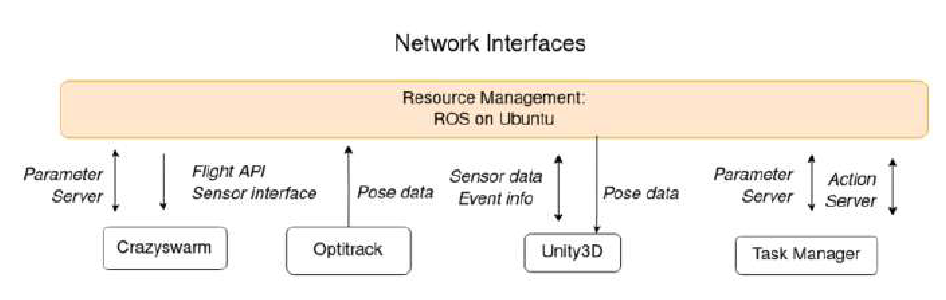
\includegraphics[width=0.5\textwidth]{images/ROSnetwork.png}}
    \caption{Drone Control Kernel developed by previous dronelab team at IFT.\cite{carstens_intelligent_nodate}}
    \label{fig}
    \end{figure} 

\subsection{Human Pose Detection for Drone Control}

Human-drone interaction has advanced with technologies that allow drones to react to human movements. One notable platform is FlyJacket, a wearable exoskeleton that translates upper body movements into drone control. FlyJacket emphasizes intuitive and immersive control, but it is focused on single-drone systems \cite{flyjacket}.

Beyond specialized wearables, recent advances in computer vision have made it possible to detect human poses and gestures without specialized hardware. Intel RealSense, combined with MediaPipe, allows real-time human pose estimation from \gls{RGB} and depth cameras. This technology can detect skeletal movements and translate them into commands for drone control \cite{realsense_mediapipe}. The system’s accuracy and low latency make it highly applicable to environments where humans and drones must coexist.

In addition, Cai et al. (2019) proposed a monocular vision system for real-time posture recognition, where drones respond dynamically to human gestures in indoor environments. This system allows for direct interaction between humans and drones but does not yet support multi-drone systems \cite{cai_human_drone}.

Leap Motion offers another avenue for gesture-based control by detecting hand and finger movements. While Leap Motion has been successfully integrated with single drones, there is still potential to expand this to swarm systems for more complex indoor tasks \cite{leap_motion}.

The paper titled \"Drone control using Kinect-based posture detection\"~\cite{realsense_mediapipe} presents a compelling approach to enhancing human-drone interaction by leveraging \gls{RGB-D} \(Red, Green, Blue-Depth\) data from the Kinect sensor. The authors demonstrate how Kinect can effectively capture real-time human poses and positions, enabling drones to respond to user gestures with a high degree of accuracy. By utilizing the depth data, the system can determine the spatial relationship between the human operator and the drone, allowing for intuitive control commands based on body movements.

This approach significantly reduces the need for additional hardware or complex controllers, as it translates natural human actions directly into drone maneuvers. The paper emphasizes that such a system can enhance the usability and accessibility of drones, particularly in indoor environments where GPS signals may be unreliable. Furthermore, the authors highlight the potential for combining this technology with other methods, such as those explored in \cite{realsense_mediapipe} and \cite{flyjacket}, to create a more robust human-drone interaction framework that addresses current limitations in the field.
% ajouter les problemes

\subsection{Gaps in Human-Swarm Interaction Platforms}
% synthese des problemes
Despite advancements in both safety mechanisms and control systems, there remains a significant gap in providing a unified platform that enables developers to control swarms of drones indoors while safely interacting with humans. Current platforms like Crazyflie and ModQuad provide scalable solutions for drone swarms but lack the necessary integration with human pose recognition and safety protocols for operating indoors around people \cite{crazyflie, modquad}. Furthermore, while platforms like FlyJacket enable human control, they focus on single-drone control, leaving a gap in swarming capabilities. 

Thus, a key challenge remains in the development of a platform that can:

    Enable real-time control of multiple drones based on human input (e.g., gestures, body movements).
    That includes real-time posture and position as all platforms do not seem to include. \cite{cflib, crazyswarm, flyjacket}
    Ensure safe flight paths in indoor environments.

    Be accessible to developers for customization and open-source integration.
        Python is accessible but we want to be able to use these drones in unity or a web service to not require client-drone connection.
	
\pagebreak
% ajouter des appindixa1 pour ajouter les traval d'Etienne Pommel en quelques paragraphes


\section{Contribution 1: Swarm Control}

\subsection{Introduction}
In this section, we present our first contribution, which is the drone control kernel. We present the software architecture that we have developed to control drones in a swarm. We also present the results of the evaluation of the drone control kernel.


We were provided a synchronous control driven \gls{API} we have worked around it to handle practial asynchronous calls. We show here this work.


\subsection{Drone Control Kernel}

\subsubsection{Introduction, Motivation and Objectives}
Currently, Crazyflie drones are controlled using their Python library, cflib, which provides developers with a robust toolkit for sending commands, receiving sensor data, and managing flight tasks. While this library offers powerful capabilities, it limits the flexibility of using the Python ecosystem, as direct access to the drones requires interacting through this specific interface. As a result, broader accessibility for developers or users unfamiliar with Python is restricted, making it challenging for people from diverse technical backgrounds to engage with drone control.

To address this limitation and open drone control to a wider audience, we propose a web-based control platform. By developing a web interface, we aim to abstract the complexities of the underlying Python-based system and make the control of drone swarms more accessible to a larger range of developers, including those familiar with other technologies. This approach democratizes drone control, allowing users to interact with Crazyflie drones through web-based \gls{API}s and interfaces, facilitating easier integration into various applications, including human-drone interactions in indoor environments.

Instantaneous \gls{API} Calls and Background Processing: Asynchronous \gls{API}s enhance the functionality of drone control applications by handling requests in the background. This approach maintains application functionality while keeping resources free to process new requests. Especially in drone operations where real-time responsiveness is crucial, this capability ensures efficient handling of multiple tasks simultaneously.

Adaptability to Connectivity and Execution Time: Asynchronous \gls{API}s are particularly beneficial in environments with variable connectivity or where requests have longer execution times. They allow for the processing of complex operations without causing delays in the application's responsiveness, crucial for real-time drone control where delay can have significant consequences.

Event-Driven Communication: Asynchronous \gls{API}s, enable more intelligent communication between internal and external services. This is especially important in drone operations where multiple events or commands may need to be handled in real time, ensuring smoother and more efficient workflows

Support for Various Protocols: These \gls{API}s support a range of messaging protocols and transports such as WebSockets and UDP subscriptions, which are essential for the dynamic and varied requirements of drone control. This flexibility allows for fast and more accessible and versatile drone operation management.
\subsubsection{Heritage and Components Used in the Project}
The drone control kernel consists of several components that work together to provide a robust and flexible control system for managing drone swarms. Crazyflie drones being used in this project communicate using the Radio component Crazy Radio PA. We include also decks that can be added to the drones to add the location of the drones using light house technology. This requires a specific deck to be added to the drones and lighthouses to be placed around the room. The drones are then able to locate themselves in the room.
\cite{carstens_intelligent_nodate}

\subsubsection{Theory}
According to the state of the art the drones can be controlled using different localization methods. The lab's legacy left us the Lighthouse positioning system. This system uses infrared light to locate the drones in space. The drones have a deck that can be added to them to allow them to locate themselves in space.

\begin{figure}[htbp]
    \centerline{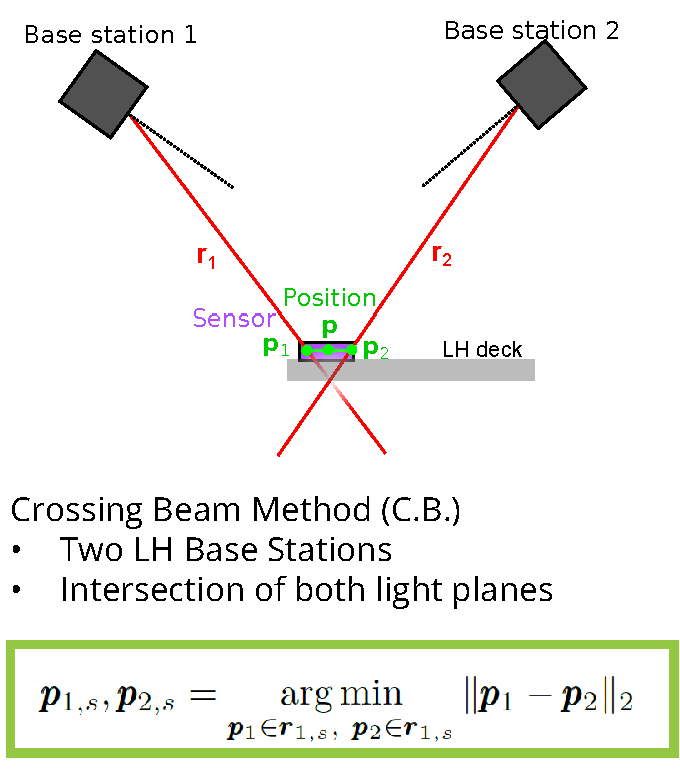
\includegraphics{images/lighthouseworking.png}}
    \caption{Drone Control Kernel, showing the workings of the Lighthouse positioning system.The idea is to calculate the vectors from two base station to a sensor on the Lighthouse deck. This vector is defined by the intersection line between the two light planes of the base station and is sometimes referred to as a “beam”, hence the name.
    In theory the beams should cross in the point where the sensor is located. In reality the point that is closest to both beams is used instead, and uses this as the estimated position. \cite{noauthor_lighthouse_nodate}}
    \label{fig}
    \end{figure}

\subsubsection{Components Evaluation}

We have evaluated the components of the drone control kernel to ensure that they meet the requirements of the system. The results of the evaluation are presented in the following sections.

We expected the drones to follow a smooth path and found that the drones were able to follow the path with a high degree of accuracy. The drones were able to maintain their position and orientation while moving along the path, demonstrating the effectiveness of the control system. 
\begin{figure}[htbp]
    \centerline{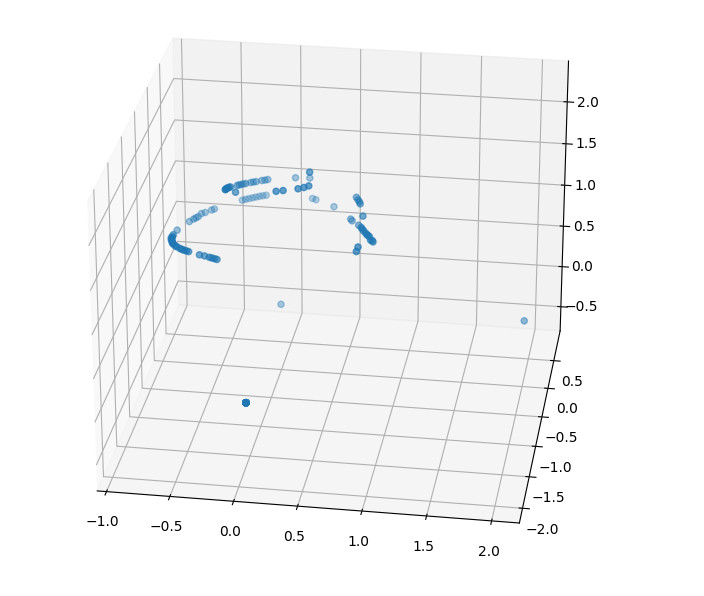
\includegraphics{images/pos.jpg}}
    \caption{Drone Components evaluation.}
    \label{fig}
    \end{figure}


\subsubsection{Architecture}
The drone control kernel is designed to provide a robust and flexible control system for managing drone swarms. The architecture of the drone control kernel is shown in Figure 1. The main components of the system are: 
Web \gls{API}, which provides the web-based interface for controlling the drones; 
Socket, which allows for lower level client drone server interface with the drones; and the Drone Control Kernel, which manages the communication with the drones using Radio. 
The UDP server runs in parallel with the Fast\gls{API} application, thanks to $asyncio.create\_task()$. \cite{asyncio} This allows the UDP server to handle datagram messages asynchronously while the FastAPI server responds to HTTP requests.

\begin{figure}[htbp]
    \centerline{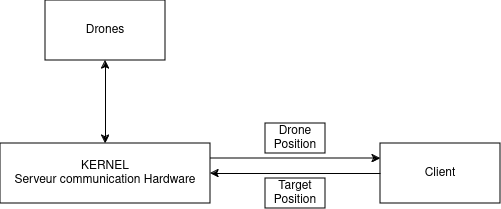
\includegraphics{images/DronecontrolKernel.png}}
    \caption{Drone Control Kernel, showing the main components of the system.}
    \label{fig}
    \end{figure}

\begin{figure}[htbp]
    \centerline{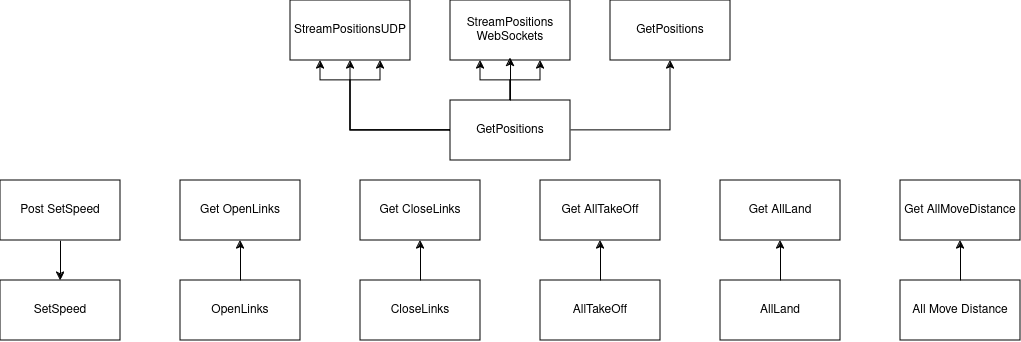
\includegraphics{images/DroneLogics.png}}
    \caption{Drone Control Kernel, inside logics.}
    \label{fig}
    \end{figure}
Using FastAPI we are able to provide a basic web based interface to control the drones. The UDP Client is used to get positions of the drones without having to wait for the drones to respond or the client to send an Acknowledgment. It is used to lower the latency of the system and to stop the package drops errors given by the TCP server on load.



Each function in the UDP server is a coroutine, which allows for asynchronous execution. The UDP server listens for incoming messages from the drones and processes them accordingly. The FastAPI application provides the web-based interface for controlling the drones. It exposes various endpoints for sending commands to the drones, such as takeoff, land, and move. The FastAPI application communicates with the UDP server to send commands to the drones and receive responses. The Socket component provides a lower-level interface for communicating with the drones using the Crazyflie Python library. It handles the connection to the drones and sends commands to them using the cflib \gls{API}. The Drone Control Kernel manages the communication with the drones using the Radio. It sends commands to the drones and receives responses from them using the Radio component (Crazy Radio PA).

Also a ThreeJS interface is provided to visualize the drones in \gls{3D} space. This interface allows users to see the drones' positions and orientations in real-time, providing a visual representation of the swarm's behavior. The ThreeJS interface communicates with the FastAPI application to receive updates on the drones' positions and orientations.
\subsection{Evaluation and Results}

We have realized that the drone control kernel had a big flaw using TCP based technologies as we would observe drops in the communication. We have then switched to UDP based technologies and have seen a big improvement in the communication. We have also seen that the drones were able to follow a path with a high degree of accuracy. The drones were able to maintain their position and orientation while moving along the path, demonstrating the effectiveness of the control system.
We werent able to break this server as we were able to send 1000 requests per second to the server and the server was able to handle them all as no function blocks the system.
This was possible because the server was made as stateless as possible. So after setup no command could break it.

There is also a big improvement in the latency of getposition requests. The TCP server would take between 0.2 and 0.5 seconds to respond to a getposition request. The UDP server is able to respond in less than 0.05 seconds using cflib low level variable accessibility. This is a big improvement in the latency of the system.
\subsection{Conclusion}

Using the drone control kernel, we have developed a robust and flexible control system for managing drone swarms. The system provides a web-based interface for controlling the drones and visualizing their positions and orientations in real-time. The system is designed to be scalable and extensible, allowing for the addition of new features and functionalities as needed. The system has been evaluated and shown to be effective in controlling drones in a swarm, with the drones able to follow a path with a high degree of accuracy using the Lighthouse positioning system. The system provides a valuable tool for developers and researchers working with drone swarms, enabling them to experiment with different control strategies and algorithms.


\section{Contribution 2: Human pose estimation Kernel}

\subsection{Introduction}
In this brief section we describe the workings of the human detection system. It was developed by Etienne Pommel for a similar use case. The system is based on the mediapipe library \cite{mediapipe2020}, which is a state-of-the-art object detection algorithm that is capable of detecting humans in real-time. \cite{realsense_mediapipe}. The system is able to detect humans with high accuracy as they move around the environment. To the standard \gls{RGB} image, the system adds depth.

\begin{figure}[htbp]
    \centerline{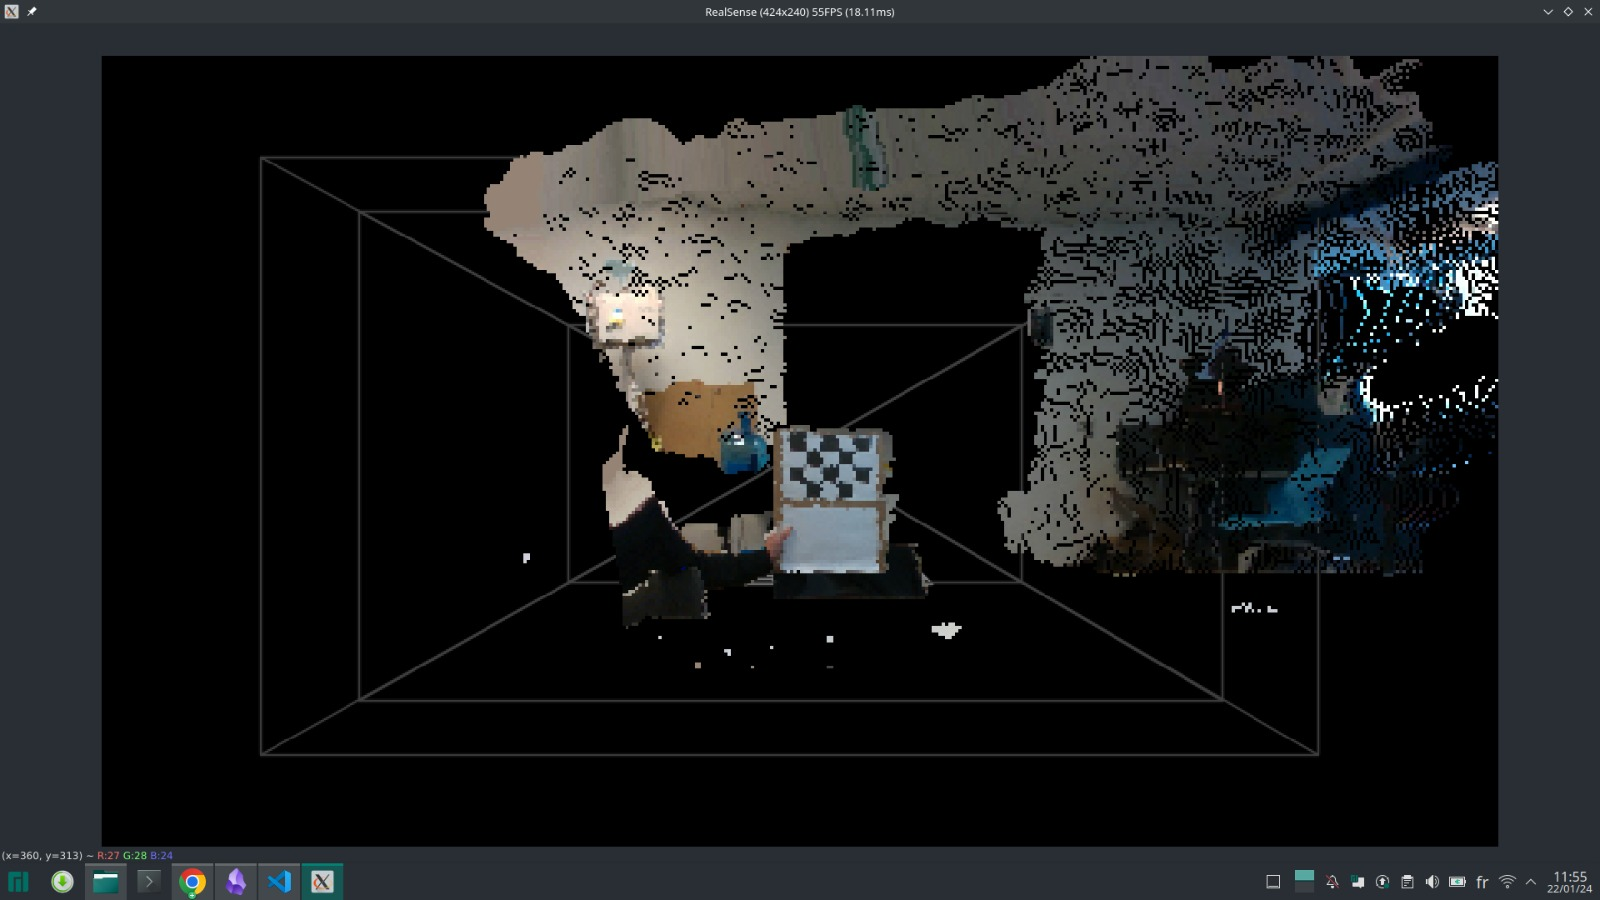
\includegraphics[width=1.0\textwidth]{images/rgbd.jpeg}}
    \caption{Intel Realsense D435, showing the workings of the depth camera and calibration capabilities, each pixel has been projected in the \gls{3D} space.}
    \label{fig}
    \end{figure} 
The difficulties of the system are to detect the objects in the image and to estimate the distance to the object. Finaly to project this distance in the \gls{3D} space.

Here we want to detect humans in the image this the use of mediapipe.

\subsubsection{Architecture}
The system was modified from the original algorithm as it would continuously calibrate using the chessboard.~\ref{appendix:additional_work}

\begin{figure}[htbp]
    \centerline{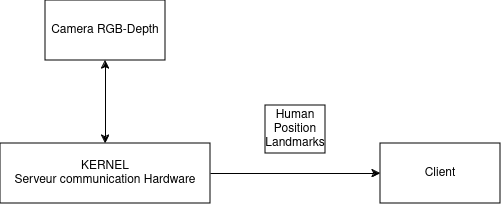
\includegraphics{images/objectschema.png}}
    \caption{Object Control Kernel, showing the main components of the system.}
    \label{fig}
    \end{figure} 
\begin{figure}[htbp]
    \centerline{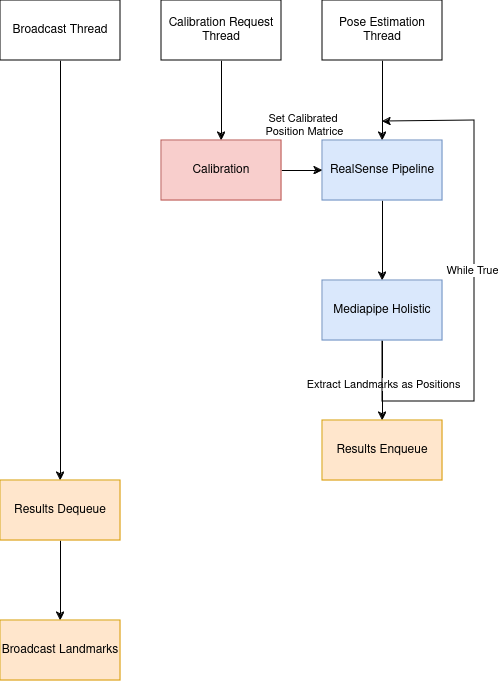
\includegraphics[width=0.5\textwidth]{images/ObjectRecognitionLogics.png}}
    \caption{Object Control Kernel, inside logics.}
    \label{fig}
    \end{figure} 

\subsection{Evaluation and Results}
Also a ThreeJS interface is provided to visualize the drones in \gls{3D} space. This interface allows users to see the humans' positions and orientations in real-time, providing a visual representation of the system's behavior. The ThreeJS interface communicates with the FastAPI application to receive updates on the humans' positions and orientations.

We have evaluated the components of the human detection kernel to ensure that they meet the requirements of the system. The results of the evaluation are presented in the following sections.

We expected the measures to be accurate to at least 5\% of the real distance but expect it to be less reliable the further the subject is to the camera. The system was not able to provide this much accuracy but 10\% at 5 meters. The system though was able to provide a good estimate of the distance to the object, constant at 2\% of the real distance at less then 7m.
\begin{figure}[htbp]
    \centerline{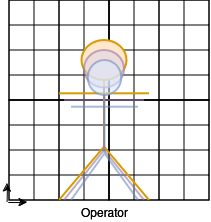
\includegraphics[width=0.3\textwidth]{images/humanreconitionflaw.png}}
    \caption{Object Control Kernel Issue, further the object is from the camera and the center of the image the smaller it will be estimated. The distance to the camera does not change only the size of the object in the image plane.}
    \label{fig}
    \end{figure} 
Indeed the results are less satisfying then expected but the system is still able to provide a good estimate of the distance to the object. The system is able to detect the object in the image and to estimate the distance to the object. The system is also able to project this distance in the \gls{3D} space, we will need to takee this into account in the next part of the project.

Similarly to the drones kernel, the system was made as stateless as possible. So after setup no command could break it. This system does not require a lot of resources and is able to send all the 30 landmarks per frame at the rate of 30 per second to the client so \[900 \text{ landmarks per second.}\]

\subsection{Conclusion} 
The human pose estimation kernel provides a valuable system for detecting and estimating the distance of humans in real-time, using the Mediapipe library in combination with depth sensors. While the results showed a degree of inaccuracy beyond 5 meters, the system successfully achieved consistent performance within 2\% accuracy for shorter distances (less than 7 meters). Despite some limitations—such as reduced reliability at greater distances and issues with object size estimation at image boundaries—the system still delivers an effective method for projecting human positions in \gls{3D} space. Future improvements should focus on enhancing the calibration mechanisms and addressing the accuracy drop at longer ranges, which will be vital for the next phase of the project.


\section{Contribution 3: Platform : Human-Swarm Interaction}
ADD IMAGE SHOWING Parallel access to services.
\begin{figure}[htbp]
    \centerline{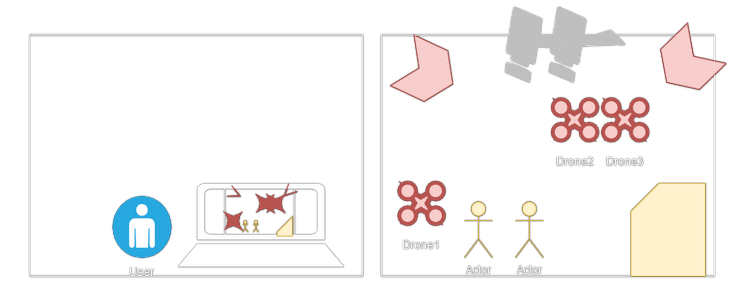
\includegraphics{images/setting.png}}
    \caption{ Our setup for controlling drones indoors around humans. }
    \label{fig}
    \end{figure}	



\subsection{Introduction}
In this section, we present our third contribution, which is the platform for human-swarm interaction. We present the setup and the software architecture that we have developed to control drones indoors around humans. We also present the results of the evaluation of the platform.

Our solution works on premise with a web-based interface to control the drones as it requires real-time computation. Both for drone control and human pose detection computation both have to be synchronized as both subjects are in the same environment. But the applications can be hosted on a cloud or other server allowing for remote control of the drones. This allows for a more flexible and scalable system.

\subsection{Platform for Human-Swarm Interaction}


Simulating drones in a virtual environment allows for the development of control algorithms without the need for physical drones. This is especially useful for testing new control strategies and algorithms in a safe and controlled environment. The platform provides a web-based interface for controlling the drones and visualizing their positions and orientations in real-time. The platform also provides a \gls{3D} visualization of the drones in the environment, allowing users to see the drones' positions and orientations in real-time. The platform is designed to be flexible and extensible, allowing for the addition of new features and functionalities as needed.
It acts as a monitoring tool for the platform. 
\begin{figure}[htbp]
    \centerline{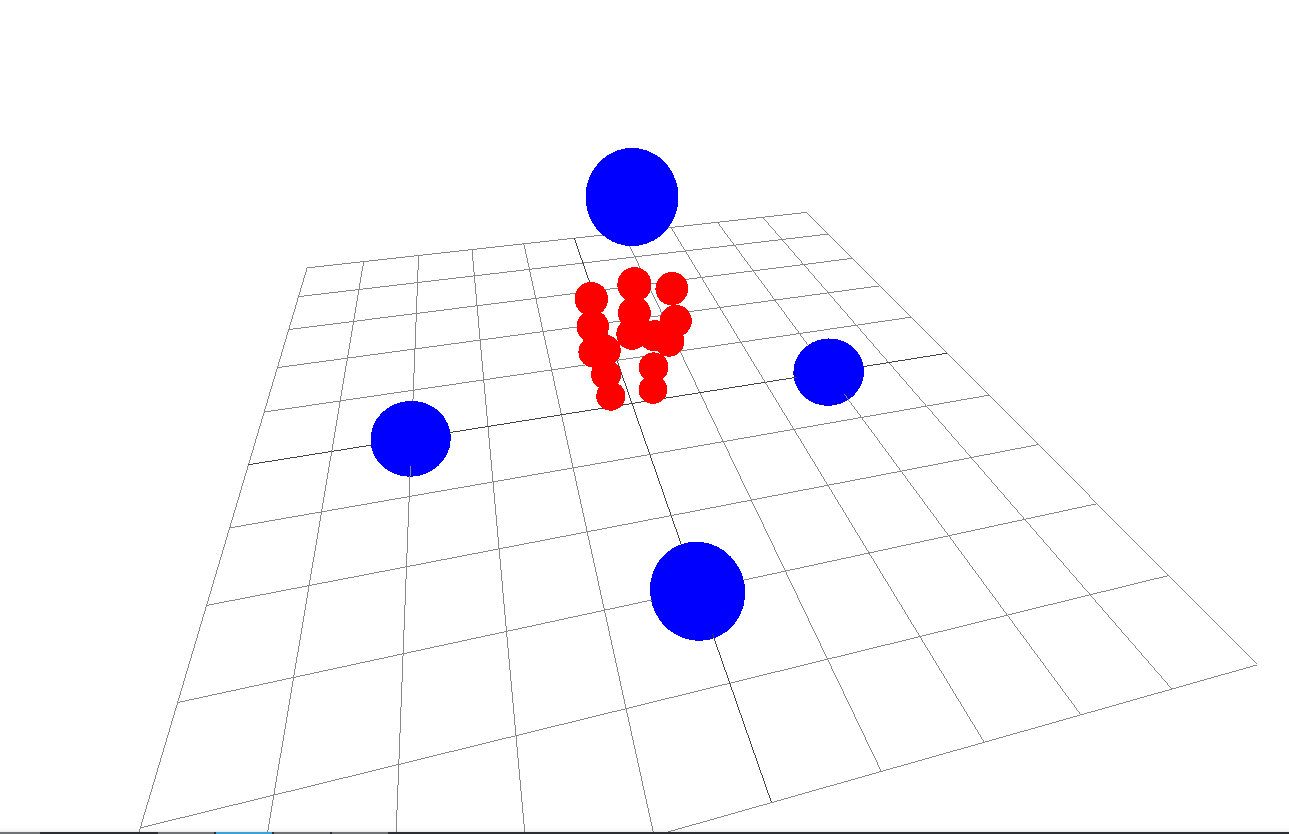
\includegraphics{images/image.png}}
    \caption{Shows the positions  of the elements of the platform through its web interface run for a few seconds.}
    \label{fig}
    \end{figure}

\begin{figure}[htbp]
    \centerline{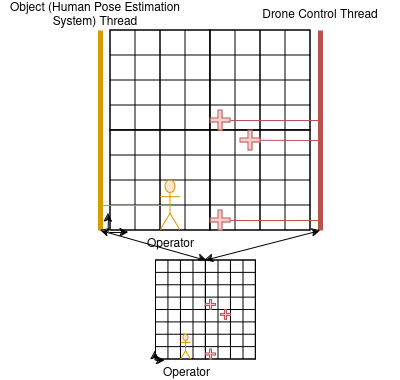
\includegraphics{images/ComboClient.png}}
    \caption{Shows the functionalities of the platform through its web interface and double threads. Above the realworld view and below the estimation after letting the system run for a few seconds.}
    \label{fig}
    \end{figure}
A user would then want to set speeds through his own app.
\subsection{Opportunitites}

As we have successfully built a usable platform with known people and subjects. We plan on testing it further and giving it to students to test further and develop on.
Students can access the platform and develop their own algorithms to control the drones and have them interact with them in real-time. This will allow students to experiment with different control strategies and learn about the challenges of controlling drones in indoor environments. Especially without having to work on the hardware part of the drones.

One student Maximilien Menesguen \cite{max} developed the famous boids \cite{reynolds1987boids} algorithm in Unity to make the drones follow a moving point in space using our UDP server, a work in progress. 
One of the main challenges in controlling drones indoors around humans is ensuring that the drones can avoid collisions with people and objects. The system continuously monitors the surroundings and adjusts the simulated drones' trajectories to avoid collisions.
it is based on the original boids algorithm. \cite{reynolds1987boids}. The boids algorithm is a simple and elegant model for simulating the flocking behavior of birds. It is based on three simple rules: separation, alignment, and cohesion. The separation rule ensures that the drones maintain a safe distance from each other, the alignment rule ensures that the drones move in the same direction, and the cohesion rule ensures that the drones stay together as a group. By following these rules, the drones can navigate the environment safely and efficiently.

The alignment rule is modified to take into account the position of the human operator so the drones interact more with the human. Thus we plan on seting the red Ball of the UAVs to be the user. This modification allows the drones to follow the human operator while maintaining a safe distance from them. The cohesion rule is also modified to ensure that the drones stay within a predefined area around the human operators. This modification would allow the drones to move around the human operator without straying too far from them.

We plan on adding the repulsion rule directly to the human operator and the drones. This rule would ensure that the drones maintain a safe distance from the human operator at all times. Adding the security layer to the platform is also a priority.

\begin{figure}[htbp]
    \centerline{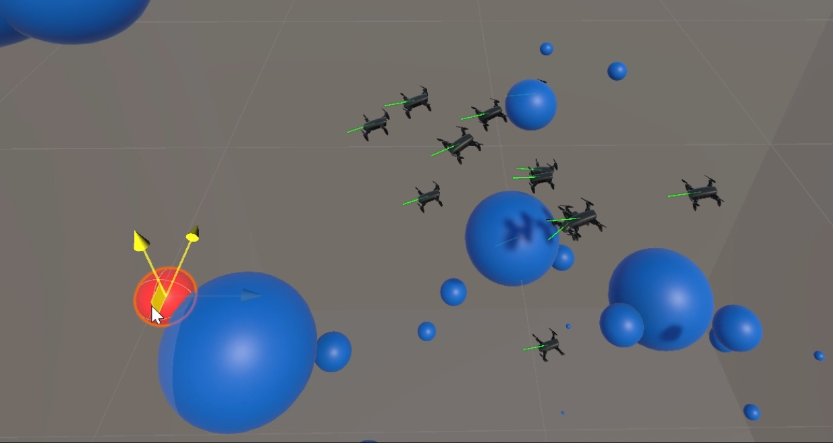
\includegraphics{images/dronesUnity.png}}
    \caption{ Drones following a moving point in space. }
    \label{fig}
    \end{figure}	




\section*{Conclusion}

This technology gives possibilities in developpement to warehouses for adding drone carriers around sensible objects or animals.

\subsubsection{Limits and Future Work}

As discussed previously in the paper, the current platform has some limitations that need to be addressed in future work. One of the main limitations is the reliance on lighthouse technology \cite{noauthor_dvic_nodate} for positioning. While it uses sensors that are effective, they are light sensitive  and may not be suitable for all indoor environments especially close to windows. Future work will focus on developing arount a more robust location system that can adapt to different environments and scenarios.

There is also a need to provide a cybersecurity layer to the platform to ensure that the drones are secure from external threats. This will involve developing a secure communication protocol to protect the drones from unauthorized access.

Finaly the platform needs to be tested in a real-world environment to evaluate its performance and reliability. This will involve conducting experiments in different indoor environments to assess the platform's intuitiveness against students. The results of these experiments will help to identify any issues with the platform and guide future development efforts.

\pagebreak

\appendix
\section{Pose etimation pipeline.}\label{appendix:additional_work}

\begin{figure}[htbp]
    \centerline{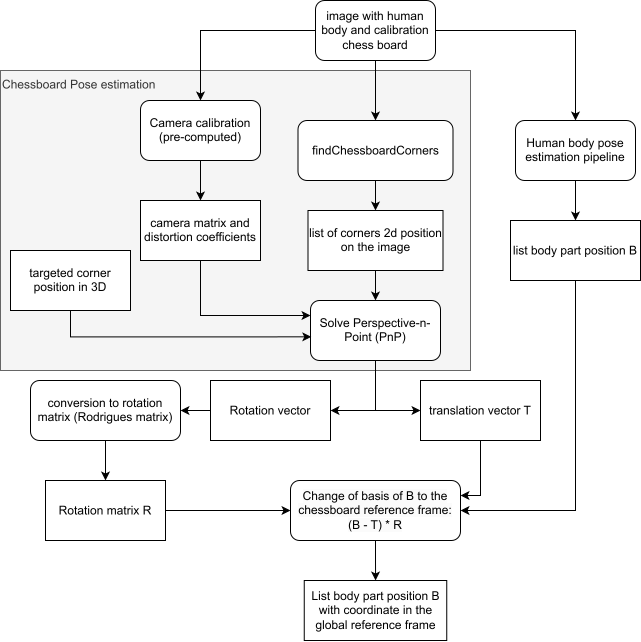
\includegraphics[width=0.5\textwidth]{images/objectcomplete.png}}
    \caption{Object Control Kernel, inside logics.}
    \label{fig}
    \end{figure} 
    The system leverages pose estimation to detect human body landmarks using computer vision, specifically OpenCV's pose estimation pipeline. First, a camera captures RGB and depth data from the environment, with the depth data being crucial for calculating the distance of each detected point. The system uses a monocular camera setup, and it processes images through MediaPipe's holistic model, which detects human body landmarks, including key body joints like the head, shoulders, and limbs. These 2D landmarks are then projected into 3D space using depth data from the RealSense camera.

    The system performs camera calibration to compute intrinsic parameters such as the camera matrix and distortion coefficients. Calibration ensures that the system accurately maps 2D pixel coordinates to real-world 3D points. OpenCV’s solvePnP function computes the human's pose (rotation and translation vectors) relative to the camera using chessboard patterns, which serve as a known reference in the scene. After obtaining the pose, the Rodrigues rotation matrix is used to transform the body landmarks into the coordinate system of the chessboard, essentially re-aligning the 3D positions of the detected human body with the physical world.
    
    This process ensures that the system can track human movement in 3D space accurately, which is crucial for human-drone interaction and control.

\pagebreak

\section*{Acknowledgment}
A Testbed Environment for Task Development was developed at
the IFT. Marc Teyssier, Xiao Xiao and Clement Duhart showed
much faith to enable such a project.

Etienne Pommel and Maximilien Menesguen of the Institute for future technologies, thank you
for joining yourselves to me. Your enthusiasm and dedication to the project have been a great source of inspiration.

Thomas Carstens and Nicolas Stas of the Institute for future technologies have been a great help in the development of the platform. Your technical expertise and guidance have been invaluable.





%----------------------------------------------------------------------------------------

\backmatter % Denotes the end of the main document content
\setchapterstyle{plain} % Output plain chapters from this point onwards

%----------------------------------------------------------------------------------------
%	BIBLIOGRAPHY
%----------------------------------------------------------------------------------------

% The bibliography needs to be compiled with biber using your LaTeX editor, or on the command line with 'biber main' from the template directory

\defbibnote{bibnote}{Here are the references in citation order.\par \bigskip} % Prepend this text to the bibliography
\printbibliography[heading=bibintoc, title=References, prenote=bibnote] % Add the bibliography heading to the ToC, set the title of the bibliography and output the bibliography note

%----------------------------------------------------------------------------------------
%	NOMENCLATURE
%----------------------------------------------------------------------------------------

% The nomenclature needs to be compiled on the command line with 'makeindex main.nlo -s nomencl.ist -o main.nls' from the template directory

% \nomenclature{$c$}{Speed of light in a vacuum inertial frame}
% \nomenclature{$h$}{Planck constant}

% \renewcommand{\nomname}{Notation} % Rename the default 'Nomenclature'
% \renewcommand{\nompreamble}{The next list describes several symbols that will be later used within the body of the document.} % Prepend this text to the nomenclature

% \printnomenclature % Output the nomenclature

%----------------------------------------------------------------------------------------
%	GREEK ALPHABET
% 	Originally from https://gitlab.com/jim.hefferon/linear-algebra
%----------------------------------------------------------------------------------------

% \vspace{1cm}

% {\usekomafont{chapter}Greek Letters with Pronounciation} \\[2ex]
% \begin{center}
% 	\newcommand{\pronounced}[1]{\hspace*{.2em}\small\textit{#1}}
% 	\begin{tabular}{l l @{\hspace*{3em}} l l}
% 		\toprule
% 		Character & Name & Character & Name \\ 
% 		\midrule
% 		$\alpha$ & alpha \pronounced{AL-fuh} & $\nu$ & nu \pronounced{NEW} \\
% 		$\beta$ & beta \pronounced{BAY-tuh} & $\xi$, $\Xi$ & xi \pronounced{KSIGH} \\ 
% 		$\gamma$, $\Gamma$ & gamma \pronounced{GAM-muh} & o & omicron \pronounced{OM-uh-CRON} \\
% 		$\delta$, $\Delta$ & delta \pronounced{DEL-tuh} & $\pi$, $\Pi$ & pi \pronounced{PIE} \\
% 		$\epsilon$ & epsilon \pronounced{EP-suh-lon} & $\rho$ & rho \pronounced{ROW} \\
% 		$\zeta$ & zeta \pronounced{ZAY-tuh} & $\sigma$, $\Sigma$ & sigma \pronounced{SIG-muh} \\
% 		$\eta$ & eta \pronounced{AY-tuh} & $\tau$ & tau \pronounced{TOW (as in cow)} \\
% 		$\theta$, $\Theta$ & theta \pronounced{THAY-tuh} & $\upsilon$, $\Upsilon$ & upsilon \pronounced{OOP-suh-LON} \\
% 		$\iota$ & iota \pronounced{eye-OH-tuh} & $\phi$, $\Phi$ & phi \pronounced{FEE, or FI (as in hi)} \\
% 		$\kappa$ & kappa \pronounced{KAP-uh} & $\chi$ & chi \pronounced{KI (as in hi)} \\
% 		$\lambda$, $\Lambda$ & lambda \pronounced{LAM-duh} & $\psi$, $\Psi$ & psi \pronounced{SIGH, or PSIGH} \\
% 		$\mu$ & mu \pronounced{MEW} & $\omega$, $\Omega$ & omega \pronounced{oh-MAY-guh} \\
% 		\bottomrule
% 	\end{tabular} \\[1.5ex]
% 	Capitals shown are the ones that differ from Roman capitals.
% \end{center}

%----------------------------------------------------------------------------------------
%	GLOSSARY
%----------------------------------------------------------------------------------------

% The glossary needs to be compiled on the command line with 'makeglossaries main' from the template directory

% \newglossaryentry{computer}{
% 	name=computer,
% 	description={is a programmable machine that receives input, stores and manipulates data, and provides output in a useful format}
% }

% Glossary entries (used in text with e.g. \acrfull{fpsLabel} or \acrshort{fpsLabel})
% Define your terms
\newglossaryentry{RGB}{
    name={RGB},
    description={Red, Green, Blue (standard color model for digital images)}
}

\newglossaryentry{RGB-D}{
    name={RGB-D},
    description={Red, Green, Blue with Depth (imaging that captures depth along with standard color)}
}

\newglossaryentry{PnP}{
    name={PnP},
    description={Perspective-n-Point (pose estimation algorithm used in computer vision)}
}

\newglossaryentry{API}{
    name={API},
    description={Application Programming Interface (a set of tools for building software)}
}

\newglossaryentry{3D}{
    name={3D},
    description={Three Dimensional}
}

\newglossaryentry{ROS}{
    name={ROS},
    description={Robot Operating System (a flexible framework for writing robot software)}
}

\newglossaryentry{cflib}{
    name={cflib},
    description={Crazyflie Library (Python-based library for drone control)}
}

\newglossaryentry{MediaPipe}{
    name={MediaPipe},
    description={A cross-platform library for real-time computer vision tasks}
}

\newglossaryentry{RealSense}{
    name={RealSense},
    description={Intel's line of depth-sensing cameras}
}

\newglossaryentry{OpenCV}{
    name={OpenCV},
    description={Open Source Computer Vision Library}
}

\newglossaryentry{Holistic}{
    name={Holistic},
    description={A pose estimation algorithm from MediaPipe for full body tracking}
}

\newglossaryentry{ML}{
    name={ML},
    description={Machine Learning}
}

\newglossaryentry{UV}{
    name={UV},
    description={Unmanned Vehicle (any type of vehicle capable of operating autonomously without a human pilot)}
}

% Define acronyms
\newacronym{JS}{JS}{JavaScript (a programming language used for web development)}

% Add acronyms to the glossary
\newacronym{UV}{UV}{Unmanned Vehicle (vehicle operating autonomously)}

\setglossarystyle{listgroup} % Set the style of the glossary (see https://en.wikibooks.org/wiki/LaTeX/Glossary for a reference)
\printglossary[title=Special Terms, toctitle=List of Terms] % Output the glossary, 'title' is the chapter heading for the glossary, toctitle is the table of contents heading

%----------------------------------------------------------------------------------------
%	INDEX
%----------------------------------------------------------------------------------------

% The index needs to be compiled on the command line with 'makeindex main' from the template directory

\printindex % Output the index

%----------------------------------------------------------------------------------------
%	BACK COVER
%----------------------------------------------------------------------------------------

% If you have a PDF/image file that you want to use as a back cover, uncomment the following lines

%\clearpage
%\thispagestyle{empty}
%\null%
%\clearpage
%\includepdf{cover-back.pdf}

%----------------------------------------------------------------------------------------

\end{document}
